\documentclass[12pt]{report}
\usepackage{amssymb}
\usepackage{multicol}
\usepackage{graphicx}
\usepackage{subfigure}
\usepackage{verbatim}
\usepackage[letterpaper,left=1cm,right=2cm, top=1.5cm,
bottom=1.5cm,head=0cm,foot=1cm]{geometry}

\parindent=0in

\newcommand{ \probDir}[1]{{ \bf\small #1 \mbox{  }}}

\newcommand{ \breakList}{\setcounter{saveenum}{\value{enumi}} \end{enumerate}}
\newcommand{ \contList}{\begin{enumerate} \setcounter{enumi}{\value{saveenum}}}


\newcounter{saveenum}

\graphicspath{ {./graphics/} }

%%%%%%%%%%%%%%%%%%%%%%%%%%%%%%%%%%%%%%%%%
\begin{document}

{\bf{Honors Physics} \hfill {Algebra Worksheet 1} \hfill {Mr. Kelley}} \\ \\
%%%%%%%%%%
\probDir{Solve the following equations for $x$:} \\
%%%%%%%%%%
\begin{multicols}{3}
\begin{enumerate}
\item $2x + 5 =  z$
\item $3x - y = 5y$
\item $5ax + 2a = -9ab$
\item $4x - 12d = 44p$
\item $z = \frac{1}{2}ax^2$
\item $\frac{3x}{7y} = 22$
\item $\frac{4y}{7x} = 16$
\item $\frac{2t}{9x} + \frac{5}{3x} = 4t$
\item $G\frac{ab}{x^2} = F$
\item $12tx + 8 = 9x$
\breakList
\end{multicols}
%%%%%%%%%%
\probDir{Write $x$ as a function of $t$:}
%%%%%%%%%%
\begin{multicols}{2}
\contList
\item $2t + 4x = 24$
\item $3t^2 + 9xt = 4t$
\item $3t^2 + 9xt = 4t -x$
\item $5t \sin x = 25 t^2$	
\breakList
\end{multicols}

\contList
\item \probDir{What is the value of $x(3)$ in the following figures?}


\begin{figure}[h]
\centering
\subfigure[]{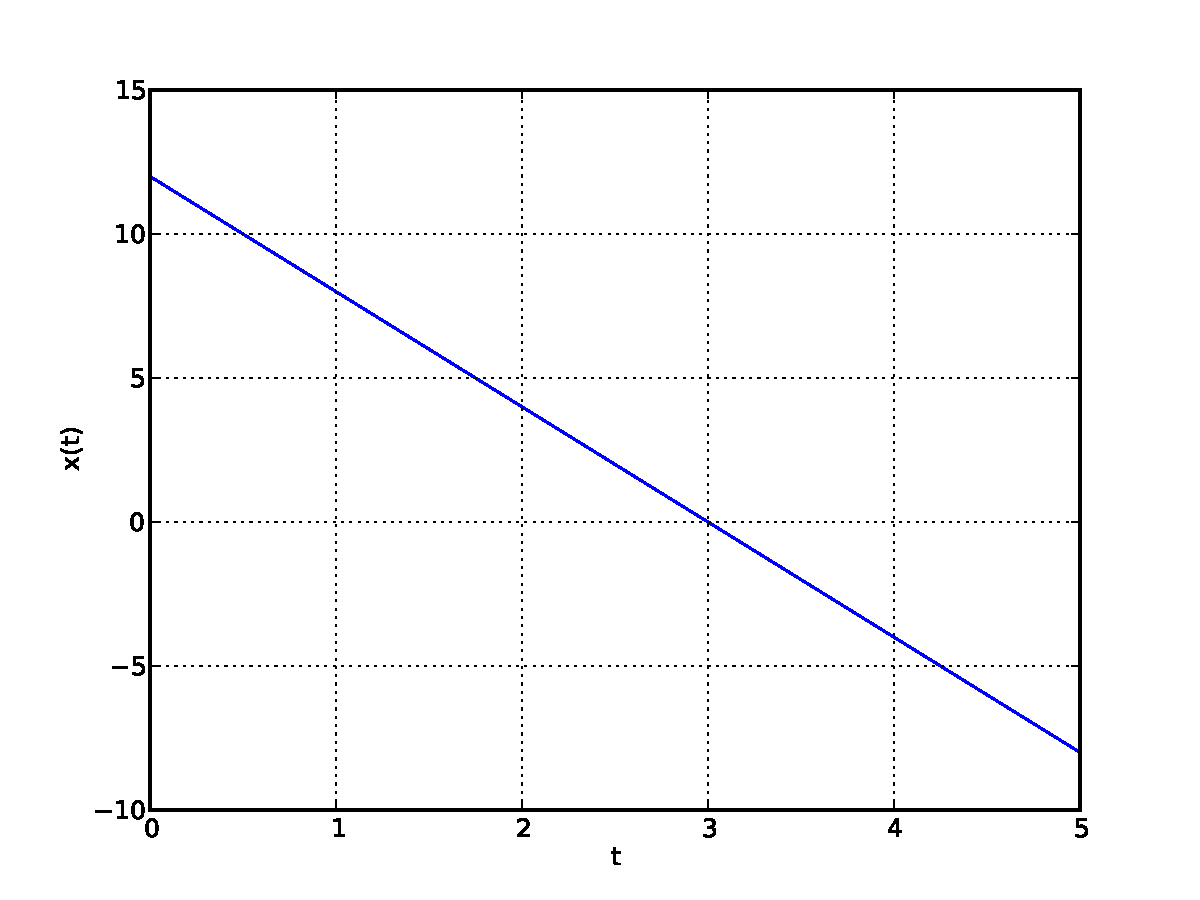
\includegraphics[scale = .45]{fig1.pdf}}
\subfigure[]{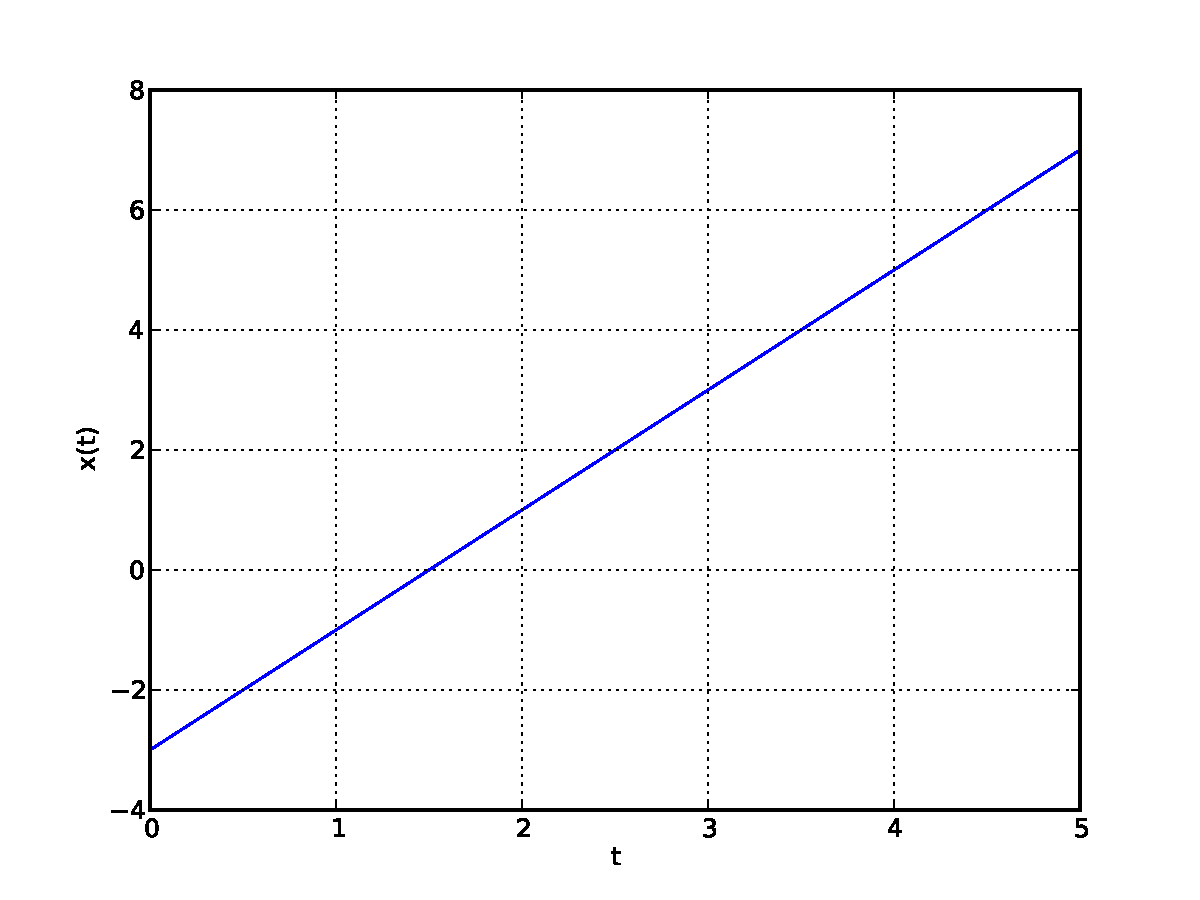
\includegraphics[scale = .45]{fig0.pdf}}
\subfigure[]{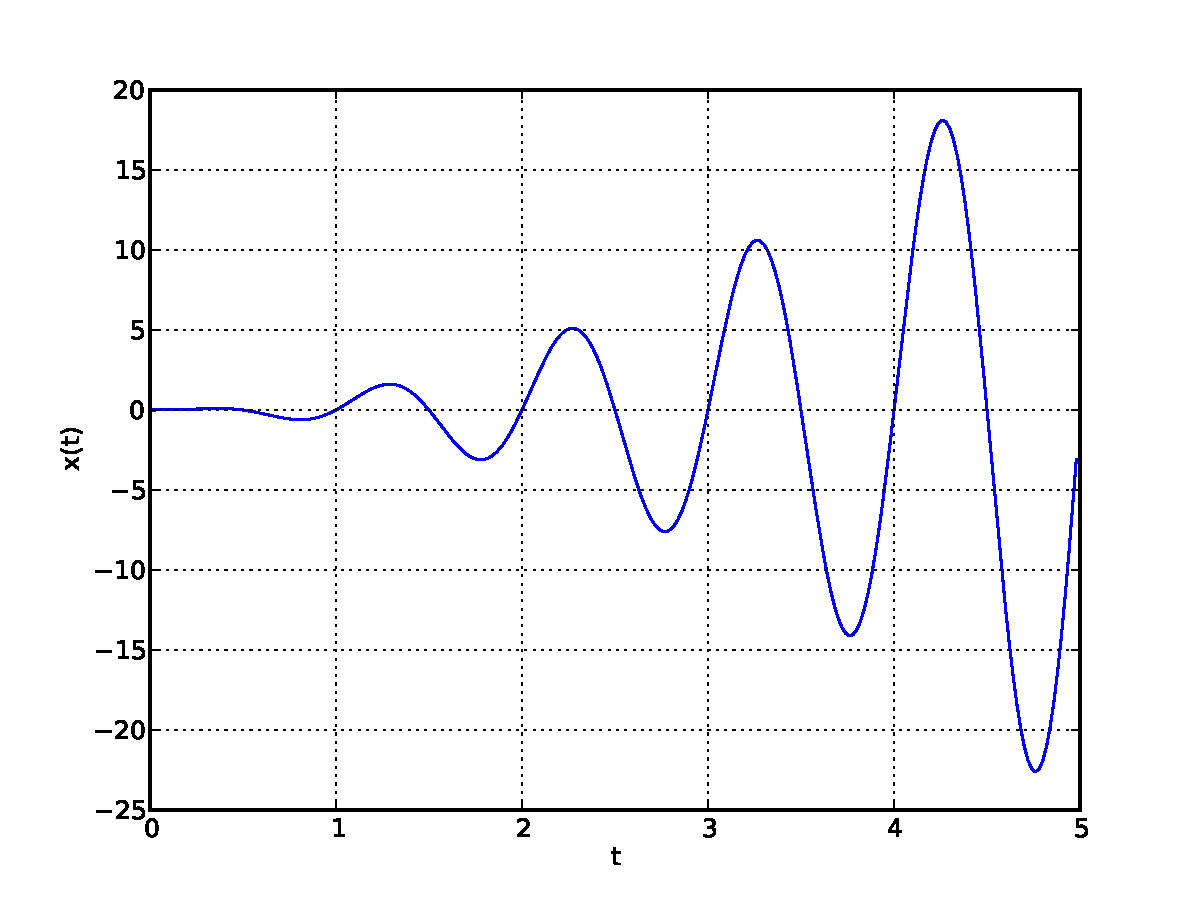
\includegraphics[scale = .45]{fig2.pdf}}
\subfigure[]{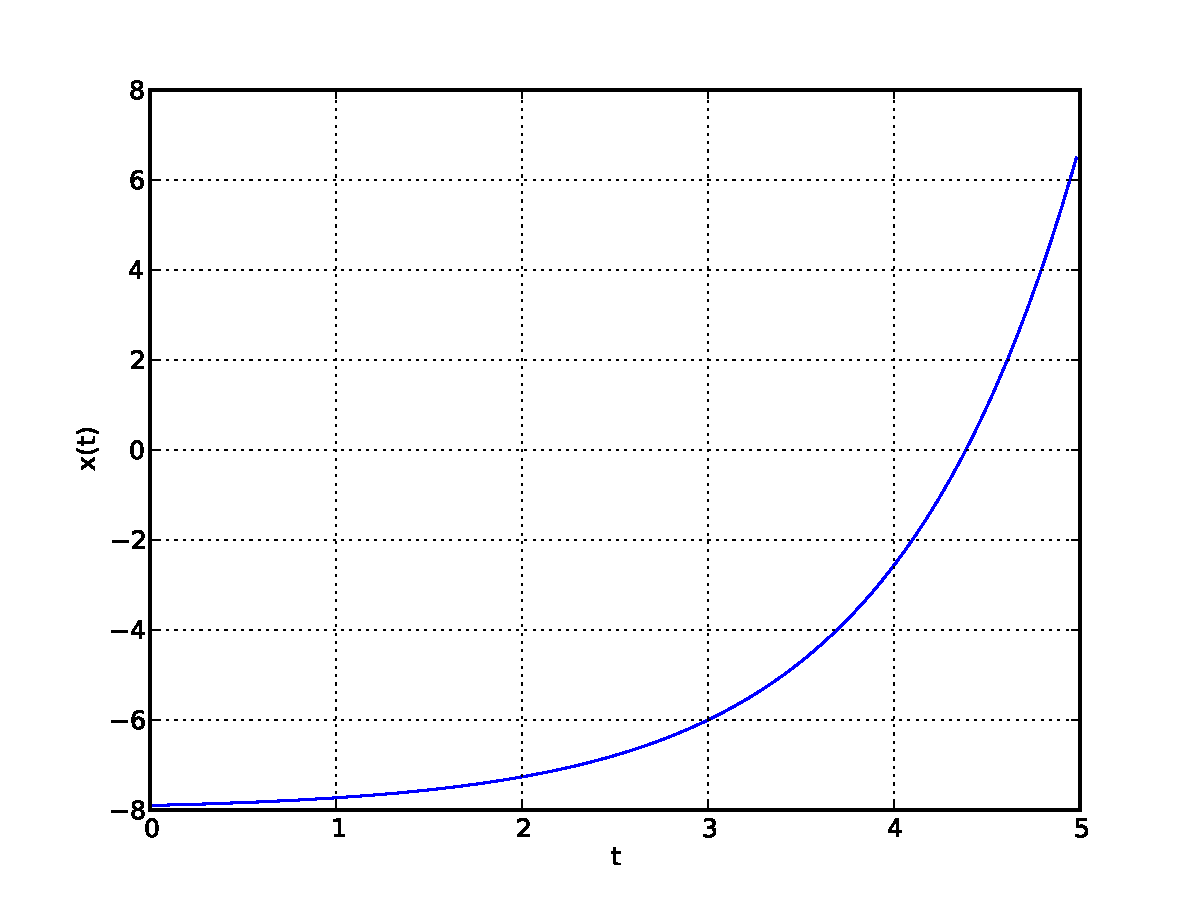
\includegraphics[scale = .45]{fig3.pdf}}
\setcounter{subfigure}{0}
\end{figure}

[more on back]

\pagebreak
%%%%%%%%%%%%%%

\item What is $x(5)$ in problem 11.
\item What is $x(0)$ in problem 12.
\item What is $x(1)$ in problem 13.
\item What is $x(-1)$ in problem 14.


\end{enumerate}

\end{document}